\section{Case Study of the Validation Procedure }\label{sec:casestudy}

In this section we apply the concepts outlined in Sec.~\ref{sec:metrics} on a simplified example of the validation procedure on an aggregator architecture similar to the one presented in \cite{thavlov2013aggregation}. While the design of these operating scenarios is outside the scope of this paper, some overall assumptions have been made. The sample aggregator name is  DTU-FlexServices, and it wants to sell ancillary services to the TSO called RisøGrid. The validation tests are carried out by the independent company AggTesters. The rest of this section presents the reference scenario, the example of the aggregator test and the evaluation process. 

\subsection{Aggregator Framework \& Portfolio}
The objective of the DTU-FlexServices is to allocate a given amount of power, provided as a setpoint by the TSO, over a controllable portfolio of 100 resistive heating systems, each providing space heating to a detached household. The objective is subject to constraints on nominal power of the heating systems and indoor comfort, which is implemented as a tolerable band in which the temperature is allowed to vary given by the interval $\left[T_{min},T_{max}\right]$. It is assumed that feedback on measured indoor temperature is available to the aggregator, such that the aggregator in real-time can assess the available capacity of the controlled heating system and ensure that indoor temperature constraints are not being violated during operation. Fig. \ref{fig:flow_diagram} presents the flow of data in the aggregator simulation framework. 
\begin{figure}[!t]
\centering
\includegraphics[width=\columnwidth]{graphics/pscc2016/flowchart.eps}
\caption{Flow diagram of the aggregator algorithm.}
\label{fig:flow_diagram}
\end{figure}
The aggregator uses a simple auto-regressive model with exogenous inputs (ARX) to assess the future available capacity of each individual households. The ARX model is given by,
\begin{equation}\label{eq:capacity}
  T_{i+1} - a\cdot T_i = b \cdot T_{a,i} + c \cdot \Phi_{s,i} + \boldsymbol{d}^T \boldsymbol{\Phi}_{h,i:i-\tau_{lag}}
\end{equation} 
where $T_i$ is the measured indoor temperature of the household at time step $i$, $T_a$ is the outdoor temperature, $\Phi_s$ is the solar irradiance and $\boldsymbol{\Phi}_{h,i:i-\tau_{lag}}$ is a vector with the most recent observed power consumptions, i.e. $\left[\Phi_{h,i},\Phi_{h,i-1} \cdots \Phi_{h,i-\tau_{lag}}\right]$. The lag parameter of the heat input, $\tau_{lag}\in\mathbb{N}_0$, is used to account for the potential time-lag that might exists between when heating is applied and when it is observed in the indoor temperature. $a$, $b$, $c\in\mathbb{R}$, and $\boldsymbol{d}\in\mathbb{R}^{\tau_{lag}+1}$ are the unknown parameters of the ARX model, which are found using prior data for power consumption of the heating system. For simplicity $\tau\equiv 0$ is assumed in the following. 

Each individual resistive heating system is assumed to be able to dispatch a continuous amount of power in the interval $\left[P_{min}, P_{max}\right]$, given by the nominal power of the heating system. Naturally, this is an approximation since resistive heating systems, in general, will only be able to dispatch power in discrete steps due the composition of resistive loads. However, considering a portfolio of many entities and following the law of large numbers, these discrete steps should level out and the assumption hold. 

To allocate the amount of power over the portfolio of resistive heating system, following unit commitment problem is formulated,
\begin{align}\label{eq:agg_dispatch}
  & \min\;\left|\; \sum_{j=1}^N \left(\Phi_{h,i,j}\right) - S_i \;\right|\; + \; \sum^{N}_{j=1}\Phi_{h,i,j}\mbox{W}\left(T_{i+1,j}\right)	\\[5mm]\nonumber
  & \mbox{s.t.} \quad P_{min,j} \leq \Phi_{h,i,j} \leq P_{max,j}  
\end{align}
where the decision variable  $\Phi_{h,i,j}\in\mathbb{R}$ is the amount of power being allocated to household $j$ at time step $i$, $N$ is the number of households in the portfolio, $S_i$ is the setpoint given to the aggregator and $\mbox{W}\left(T_{i+1,j}\right)$ is a weight function of the predicted indoor temperature found from Equation \eqref{eq:capacity}. The weight function should be constructed such that $\mbox{W}\left(\cdot\right)<-1$ for $T_{i+1,j} < T_{min}$, thus making the last term dominate the cost function and force the allocated power up for household $j$. Likewise, $\mbox{W}\left(\cdot\right)>1$ for $T_{i+1,j} > T_{max}$, thus forcing the power down. Following linear weight-function is proposed,
\begin{equation}\label{eq:weight_fct}
  \mbox{W}\left(T_{i+1,j}\right) = \frac{2\left(T_{i+1,j}-T_{min,j} \right)}{T_{max,j} - T_{min,j}}-1 
\end{equation}
The simulation model of the individual households is implemented as a stochastic linear state space model in discrete time, which is     given by
\begin{align}\label{eq:simulation_model}
  \boldsymbol{T}_{i+1} &= \boldsymbol{A}\boldsymbol{T}_i + \boldsymbol{B}\boldsymbol{U} + \boldsymbol{\sigma}_i \\\nonumber
  T_i &= \boldsymbol{C}\boldsymbol{T} + e_i
\end{align}
where $T_i\in\mathbb{R}$ is the locally measured indoor temperature which is assumed to be forwarded to the aggregator, $\boldsymbol{T}_i\in\mathbb{R}^n$ is the state vector and $\boldsymbol{U}\in\mathbb{R}^m$ is the input vector. $\boldsymbol{A}\in\mathbb{R}^{n\times n}$, $\boldsymbol{B}\in\mathbb{R}^{n\times m}$ and $\boldsymbol{C}\in\mathbb{R}^{1\times m}$ are the system, input and output matrix, respectively. To account for unrecognized input and approximations, process noise, $\boldsymbol{\sigma}_i\in\mathbb{R}^n$, is added to the system equation, \eqref{eq:simulation_model}. In the following, $\boldsymbol{\sigma}$ is assumed to be a Gaussian white noise process. Furthermore, $n\equiv1$ is assumed, i.e. only one temperature state is being simulated in the households; hence, since a Gaussian white noise process is fully characterized by its variance, the process noise is fully described by the variance $\sigma\in\mathbb{R}$.% Naturally, a single state would not be sufficient for thermally heavy households with multiple heat reservoirs, e.g. households with floor heating.

The aggregator framework and simulation models, simulating the considered scenario, have been implemented in \textsc{matlab} and is presented in full detail in \cite{thavlov2013aggregation}. It is important to note that the aggregator is described in this section for the purpose of the paper, but this description is contained within the conceptual black box described in Sec.~\ref{subsec:assumptions}, and the testing entity only has access to the general composition of the aggregator portfolio.

\subsection{Service Requirements, Normal Operation and Operation Scenario}\label{subsec:scenario}
The DTU-FlexServices aggregator wants to participate in the ancillary service markets with a FRR up-regulation service with a volume of 250 kW. 
Since it is the first time DTU-FlexServices participates in the market for this service, RisøGrid requires DTU-FlexServices to go through the validation process. Following the steps outlined in Sec.~\ref{sec:alignment}, the validation process consists of the following steps:
\begin{enumerate}
\item DTU-FlexServices presents the documentation for its portfolio.
\item RisøGrid sets the test service requirements as:
    \begin{itemize}
        \item Response accuracy:  $E[RMS] \leq 60\,kW$
        \item The response durations: $\tau = 1\,h$
    \end{itemize}
\item AggTesters identifies the normal operation scenario as:
    \begin{itemize}
        \item One source of uncertainty is the availability of the portfolio, which is a uniform distribution between 70\% and 100\%. This also accounts for minor changes in the portfolio size.
        \item A second source of uncertainty is in the disturbances induced by unrecognized user behavior and inaccurate weather forecast in the house simulation model. This uncertainty is described by $\sigma$ in Eq.~\eqref{eq:simulation_model}.
    \end{itemize}
\end{enumerate}

\subsection{Aggregator test}
To test for different combinations of the two sources of uncertainties, a series of simulations are carried out with permutations of the two. Assuming the availability to be uniformly distributed, the tests are carried out in discrete steeps across the 70\% -- 100\% spectrum of availability. Likewise, the variance of the noise process is tested in discrete steps in the 0.00 -- 0.30 domain. Fig.~\ref{fig:test100} and Fig.~\ref{fig:test70} present the outcome of two different simulations for 100\% and 70\% availability, respectively, and $\sigma=0.10$. Each permutation of the two noise sources is simulated 100 times.
\begin{figure}[!t]
%\centerline{
\centering
\subfloat[Response accuracy]{\includegraphics[width=0.85\columnwidth]{graphics/pscc2016/agg_power_ctrl_100SH_0STATIC_05PCT_REDUCTION.eps}%
\label{fig:ref100}}
%\vfill
\\
\subfloat[House Temperatures]{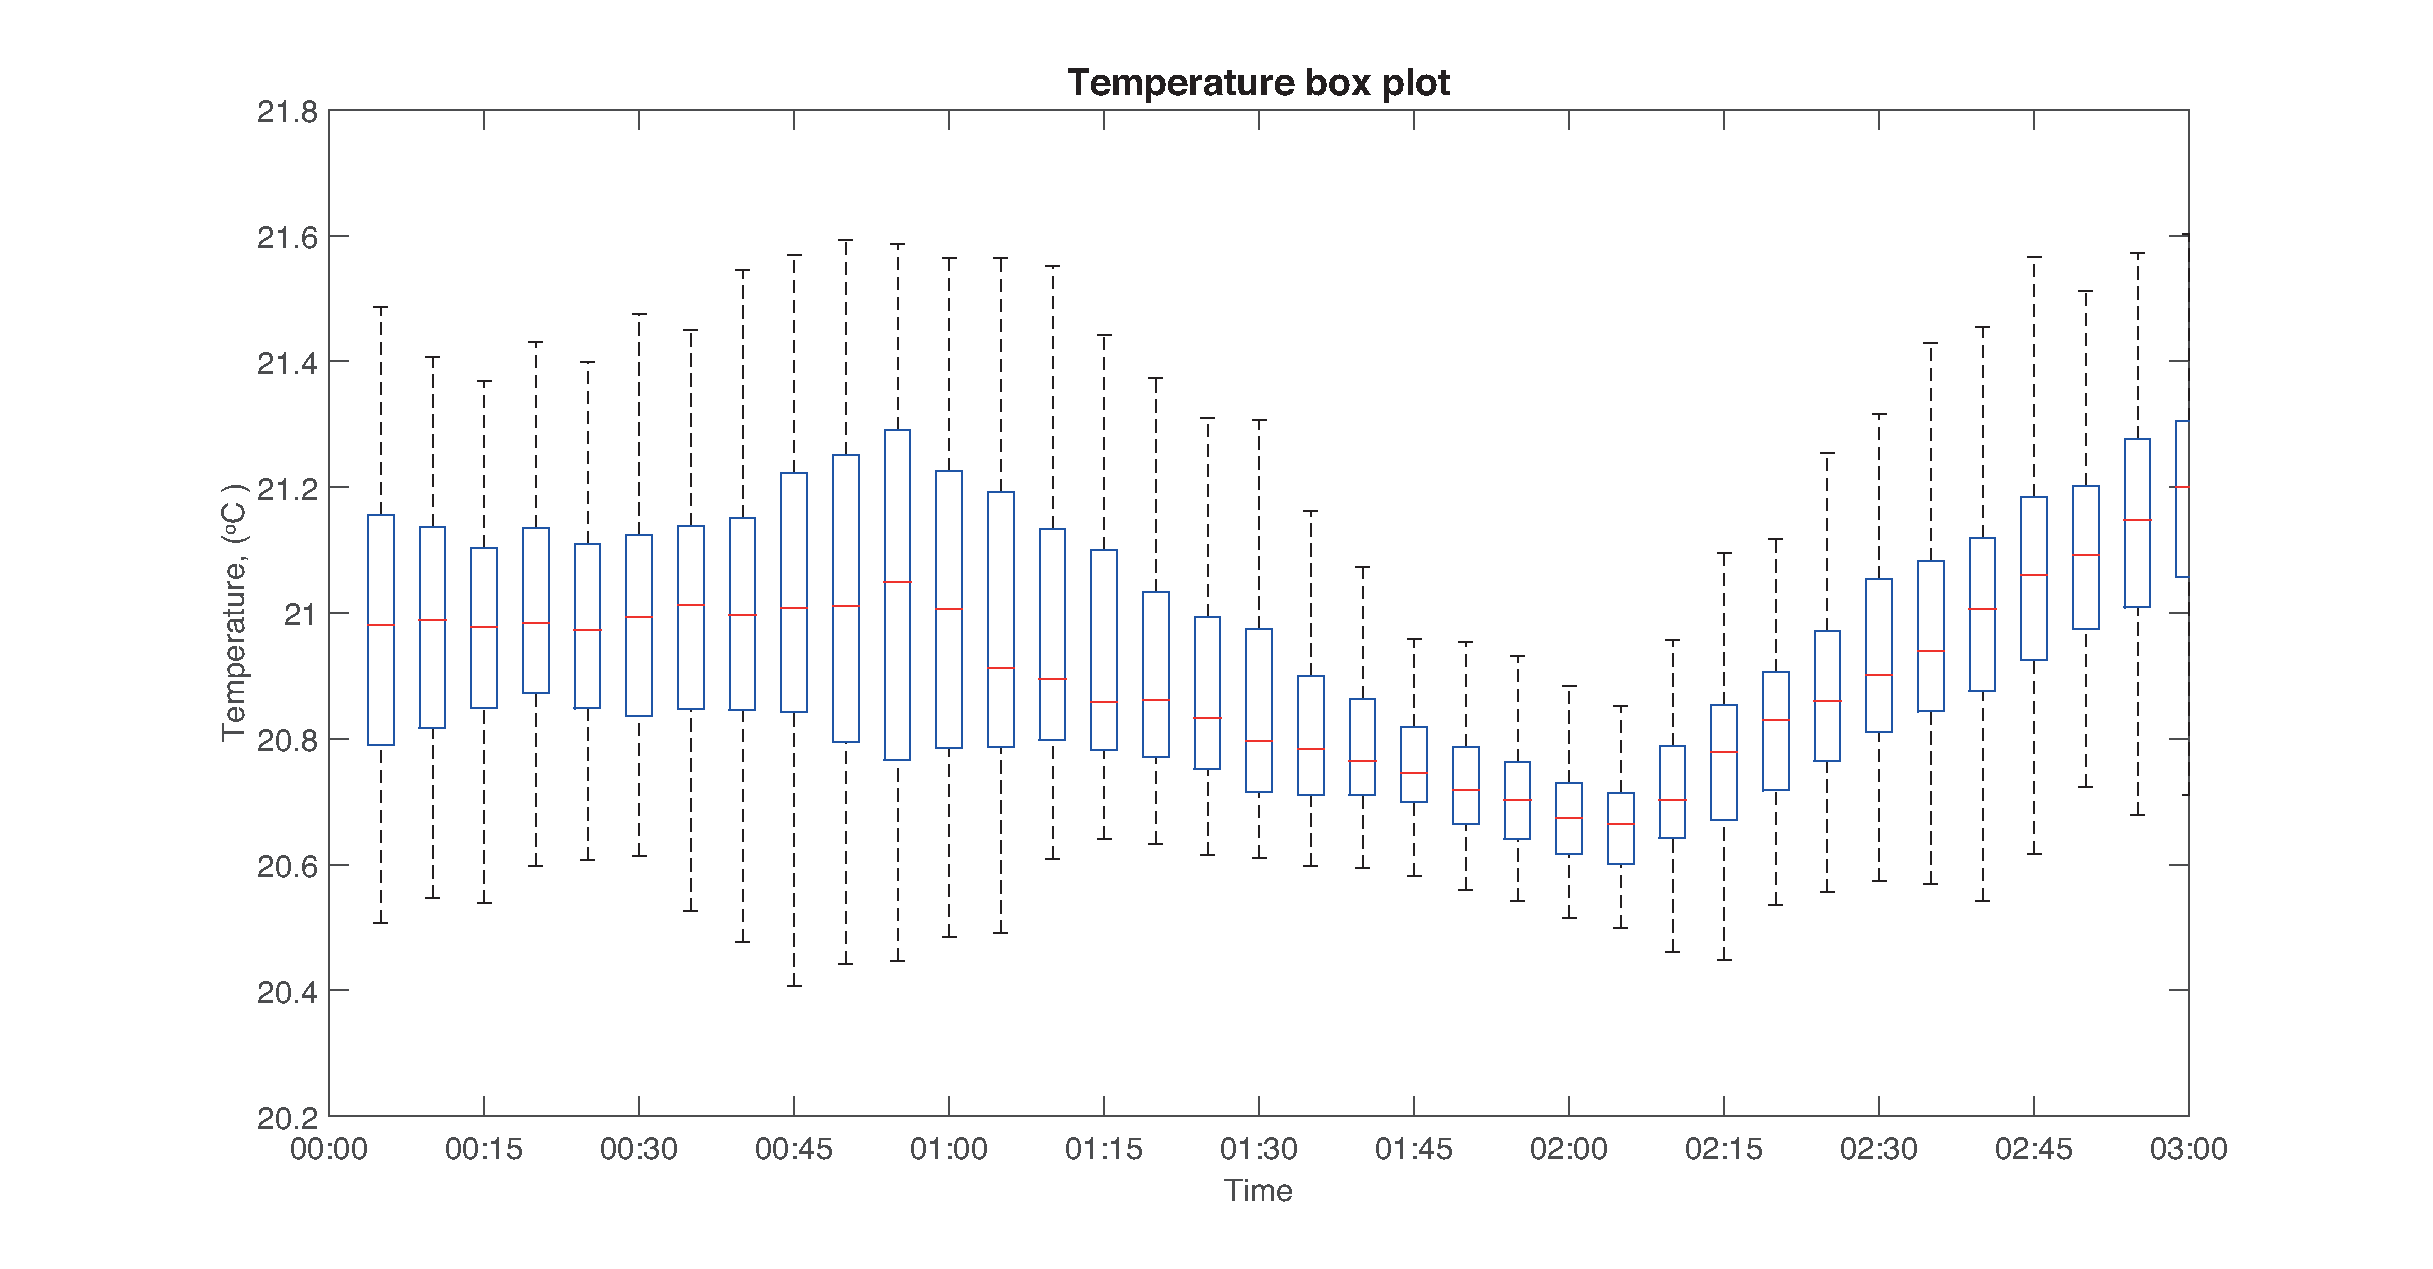
\includegraphics[width=\columnwidth]{graphics/pscc2016/agg_box_plot_100SH_0STATIC_05PCT_REDUCTION.eps}%
\label{fig:temp100}}%}
\caption{Simulation results of the 100\% availability test for the whole portfolio.}
\label{fig:test100}
\end{figure}

\begin{figure}[!t]
%\centerline{
\centering
\subfloat[Response accuracy]{\includegraphics[width=0.85\columnwidth]{graphics/pscc2016/agg_power_ctrl_70SH_30STATIC_05PCT_REDUCTION.eps}%
\label{fig:ref70}}
%\vfill
\\
\subfloat[House Temperatures]{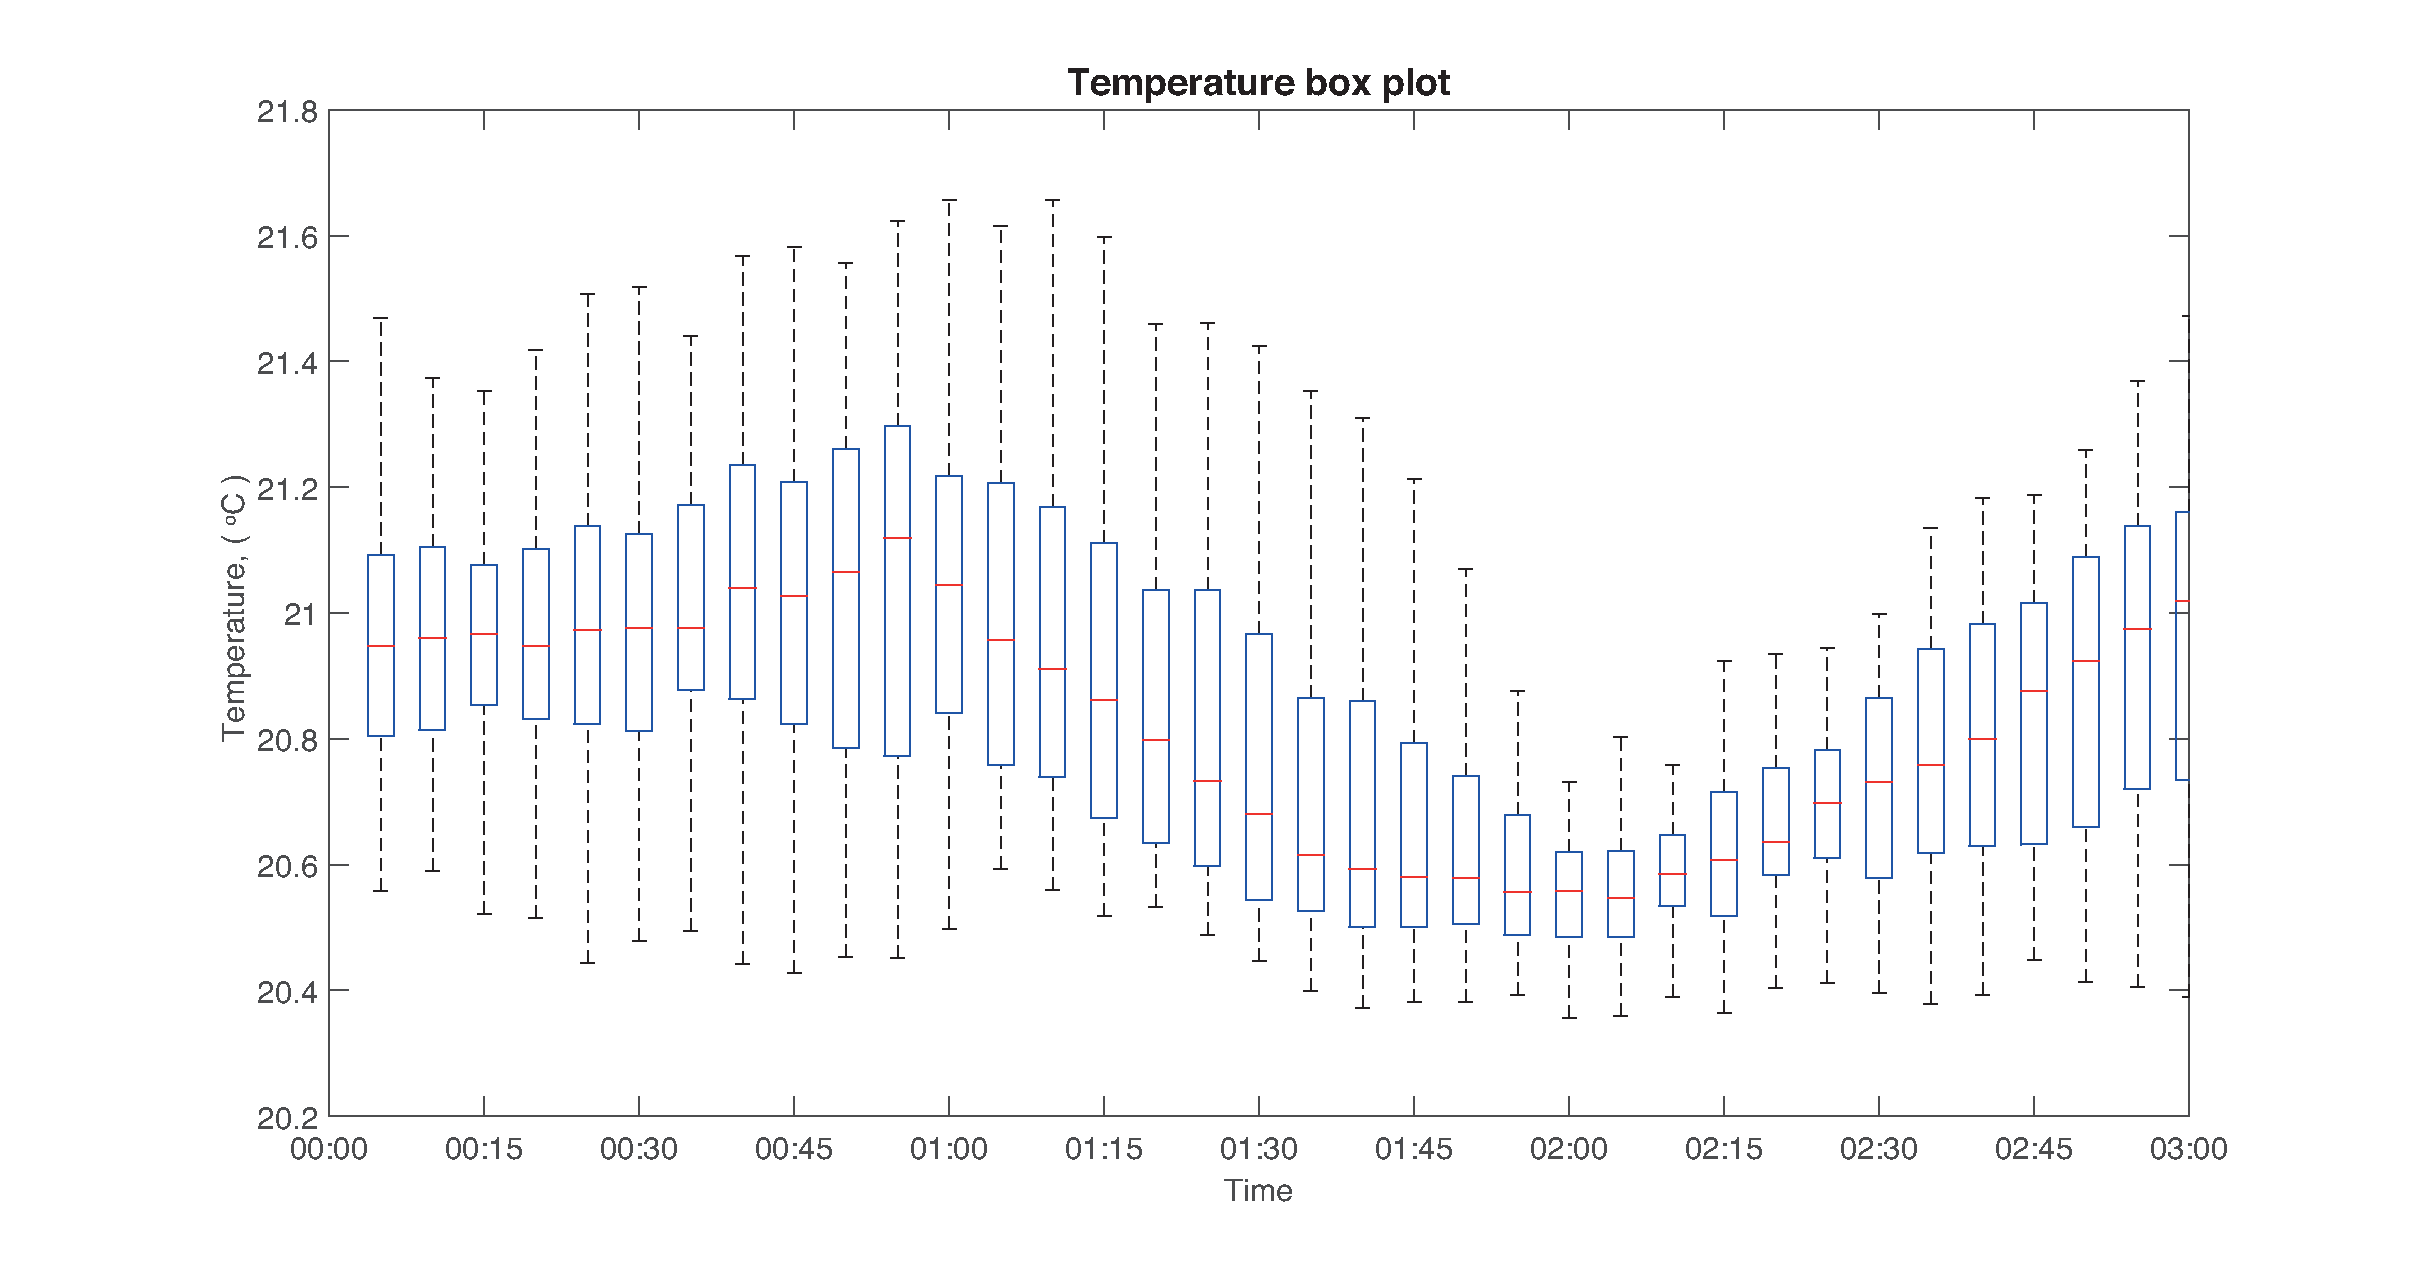
\includegraphics[width=\columnwidth]{graphics/pscc2016/agg_box_plot_70SH_30STATIC_05PCT_REDUCTION.eps}%
\label{fig:temp70}}%}
\caption{Simulation results of the 70\% availability test for the whole portfolio}
\label{fig:test70}
\end{figure}

The response accuracy of DTU-FlexServices and the average temperature of its portfolio can be seen in Fig.~\ref{fig:ref100} and Fig.~\ref{fig:ref70}. The distribution of the house temperatures can be seen in Fig.~\ref{fig:temp100} and Fig.~\ref{fig:temp70}, and it is clear that as the availability of the houses decreases, the flexibility for up-regulation is being saturated faster and the DTU-FlexServices is unable to track the FRR reference signal.

Having carried out the necessary test, RisøGrid proceeds to evaluate the results of the tests.

\subsection{Evaluation of test results}
Since the case study looks at simplified setup, and the example does not take the time responsiveness metric into account, it does not make sense to use the aggregator performance metric mentioned in Sec.~\ref{sec:evaluation}. In Sec~\ref{subsec:scenario}, the root mean square (RMS) error is chosen to measure the response accuracy metric: 
\begin{equation}
  \eta_{RMS} = \sqrt{\frac{1}{M}\sum_{i=1}^M\left(\sum_{j=1}^N\left(\Phi_{h,i,j}\right) - S_i\right)^2}
\end{equation}
where $\left[1,M\right]$ are the iterations where the aggregator has been activated. The results of the test are presented in Table~\ref{tab:results}, where it can be seen that $E[\eta_{RMS}]<60 \, kW$. Therefore the DTU-FlexServices is certified to provide FRR up-regulation service to RisøGrid.

\begin{table*}[!t]%% increase table row spacing, adjust to taste
\renewcommand{\arraystretch}{1.1}
% if using array.sty, it might be a good idea to tweak the value of
% \extrarowheight as needed to properly center the text within the cells
\caption{Performance of DTU-FlexServices}
\label{tab:results}
\centering
% Some packages, such as MDW tools, offer better commands for making tables
% than the plain LaTeX2e tabular which is used here.
\begin{tabular}{clcccccccc}
\toprule
        & & \multicolumn{7}{c}{Process noise, $\sigma$}                   & Average \\
        & & 0.00   & 0.05   & 0.10   & 0.15   & 0.20   & 0.25    & 0.30   &         \\ 
\midrule
\multirow{7}{*}{\rotatebox[origin=c]{90}{Availability}} 
& 100\%   & 0.00   & 0.00   & 0.04   & 9.25   & 31.20  & 48.84   & 98.32  & 26.81   \\
& 95\%    & 0.03   & 0.00   & 1.51   & 19.19  & 37.97  & 66.56   & 102.05 & 32.47   \\
& 90\%    & 1.40   & 0.04   & 14.36  & 30.78  & 58.74  & 73.38   & 98.24  & 39.56   \\
& 85\%    & 1.10   & 35.23  & 4.06   & 45.28  & 83.06  & 83.40   & 115.11 & 52.46   \\
& 80\%    & 13.88  & 29.25  & 12.94  & 65.93  & 72.31  & 94.50   & 135.85 & 60.67   \\
& 75\%    & 54.28  & 40.74  & 39.91  & 75.22  & 86.14  & 114.13  & 135.76 & 78.03   \\
& 70\%    & 45.63  & 90.90  & 85.41  & 99.02  & 93.68  & 123.82  & 142.64 & 97.30   \\
\midrule
Average & & 16.62  & 28.02  & 22.60  & 49.24  & 66.16  & 86.38   & 118.28 & 55.33   \\
\bottomrule
\end{tabular}
\end{table*}
%\begin{figure}[!t]
%\centering
%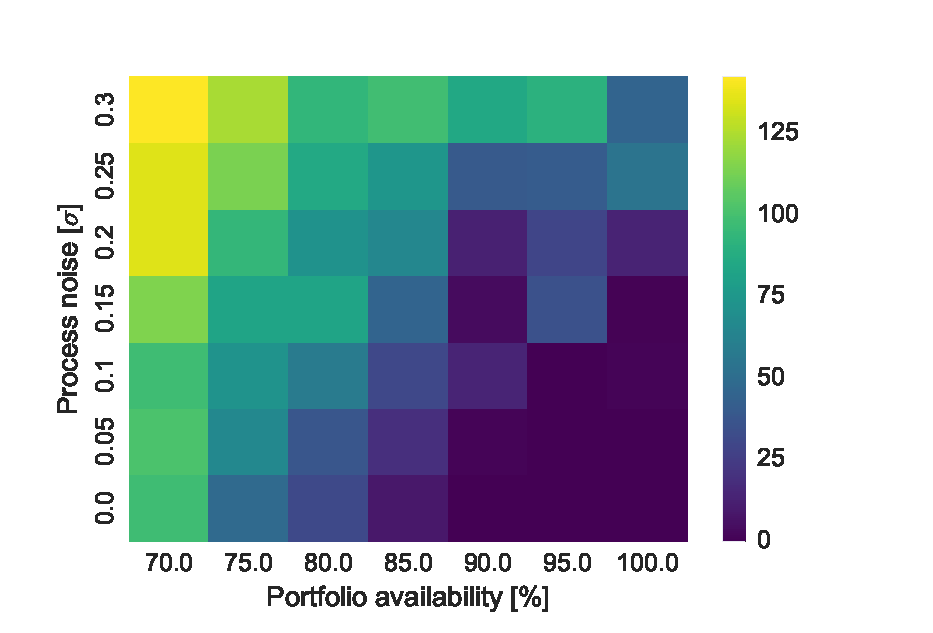
\includegraphics[width=\columnwidth]{figures/heatmap.eps}
%\caption{The RMS value over the test space. It can be seen that it is more important to have certainty in the portfolio availability than in the process noise.}
%\label{fig:colormap}
%\end{figure}
